%% objective
%Using the modENCODE developmental data \citep{Graveley2011}, with expression data for 30 stages of the whole life cycle of \textit{D. melanogaster} (12 embryonic at 2-h intervals for 24 h, 6 larval, 6 pupal and 3 sexed adult stages at 1, 5 and 30 days after eclosion), $\omega_{\alpha}$ and other evolutionary rates for the genes expressed in each stage (for details see: IV, methods) were estimated.
%For each stage, $\omega_{\alpha}$, $\omega$, $\omega_{d}$ and $\alpha$ (Fig. \ref{fig:Art-IV-OmegaA_lifecycle}) were estimated with the differentially expressed genes (genes with expression different from zero and excluding those expressed in all stages).
%Also, different "genomic determinants" (e.g., codon usage bias, intron length, or number of exons) were estimated for each stage, in order to test how their temporal patterns would relate to the temporal patterns of the estimated evolutionary rates (i.e., $\omega_{\alpha}$, and others).

%% results OmegaA

\subsection{Temporal adaptation profile}

The results of the adaptation analysis through the life cycle of \textit{D. melanogaster} show a clear temporal pattern, in which $\omega_{\alpha}$, $\omega_{d}$ and $\omega$ show their highest value at the first embryo stage (0-2hr) to then decrease until the 10-12hr embryo stage and remain low through most of embryonic development.
% (the embryonic period were briefly discussed in section \ref{OmegaA_late_embryo}).
Then, from larval stage L3 the values increase and remain relatively high through all the pupa. Finally, in the adult stages, males show similar values to those of the pupa, but females show significantly lower values (p < 0.001).  
$\alpha$ follows a similar temporal profile to that of $\omega_{\alpha}$, but the differences in $\alpha$ values through the life cycle are smaller than those of $\omega_{\alpha}$.
%
The pupal and adult male stages exhibit the highest levels of adaptive, which is consisted with previously reported higher adaptive substitutions in the genes expressed in males \citep{Proschel2006,Haerty2007}.

In summary, the results show that adaptation evidence in two different periods: 1) in the earliest 2 hours of the embryo development and 2) from the L3 larval stage onwards, while mid and late embryonic stages show high conservation. 
Similar results were found when considering after excluding immune system and testes genes (IV, Fig. S2) or when the mutation rate is estimated using the 4-fold degenerate sites (IV, Fig. S3).

%%%%%%%%%%%%%%%%%%%%%%%%%%%%%%%%%%%%%%%%%%%%%%%%%%%%%%%
\begin{figure}[t]
  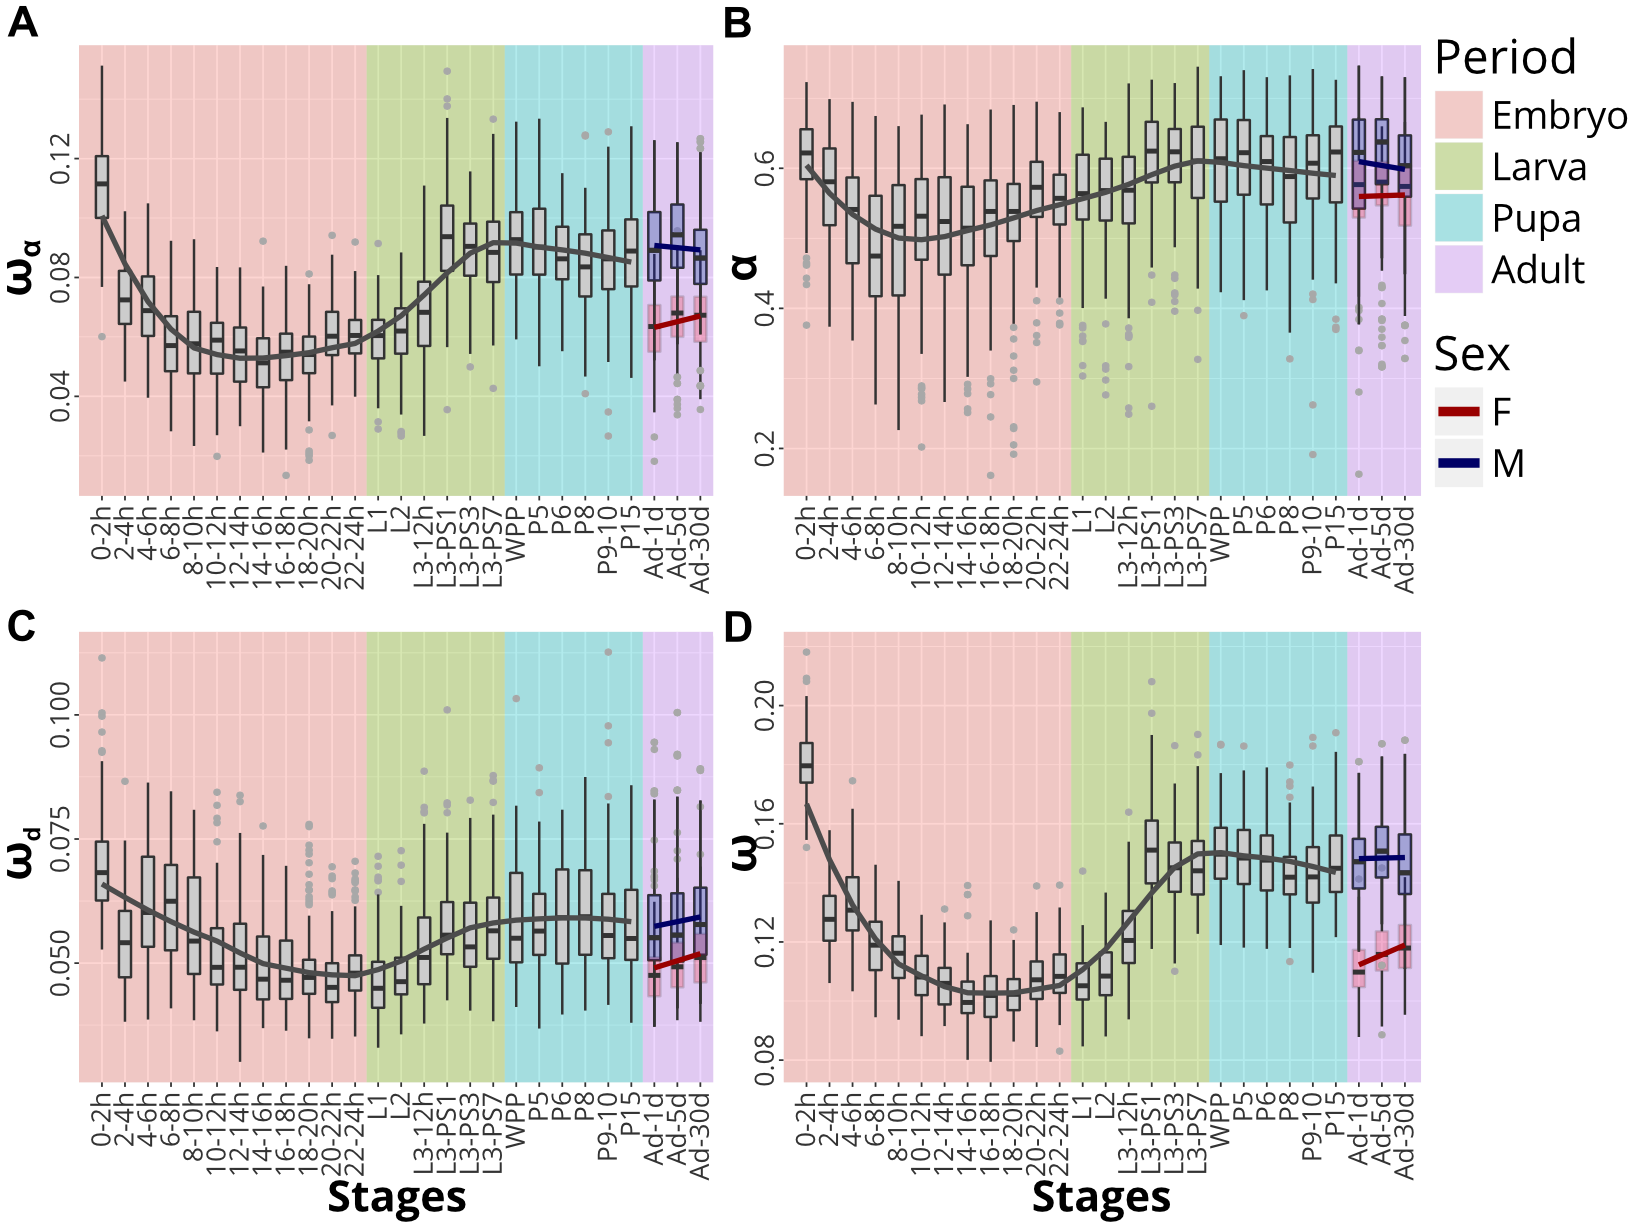
\includegraphics[width=0.9\textwidth]{./Images/Art-IV/OmegaA_lifecycle.png}
  \centering
  \caption{\textbf{ {\large$\omega_{\alpha}$} (A),  {\large$\alpha$} (B), {\large$\omega_{d}$} (C), {\large$\omega$} (D) through the life cycle of \textit{D. melanogaster}} Each time point represents 1,000 random samples of 350 genes (with replacement) expressed in a stage. Red line represents a LOESS regression. Female and male stages are fitted to a linear regression. There are 12 embryonic stages at 2hr intervals (from 0h to 24h). Larval stages at first instar (L1), second instar (L2) and third instar (L3). L3 stages are subdivided into the first 12 hours (L3-12h) and several puff stage (L3-PS1 to L3-PS7). WPP is the white pre-pupae stage. Pupal stages are phanerocephalic pupa, 15h (P5), 25.6 hours pupa (P6), yellow pharate, 50.4 hours (P8), amber eye-pharate, 74.6 hours (P9-10), green meconium pharate, 96 hours (P15). Adult stages are 1, 5 and 30 days after eclosion (Ad-1d, Ad-5d, Ad-30d).
  }
  \label{fig:Art-IV-OmegaA_lifecycle}
\end{figure}
%%%%%%%%%%%%%%%%%%%%%%%%%%%%%%%%%%%%%%%%%%%%%%%%%%%%%%%%

%% result genomic determinants
\subsection{Correlation of adaptation with some genomic determinants}
Many "genomic determinants" temporal profile correlate either positively other negatively with $\omega_{\alpha}$ (IV, Figs 2 and 3). 
%
Thus, messenger complexity (number of transcripts divided by the number of exons) correlates with $\omega_{\alpha}$, whether if comparing males or females (rank correlation; see study IV).
On the contrary, gene size, number of exons, codon usage bias and number of transcripts per gene negatively correlate with $\omega_{\alpha}$, whether if comparing males or females (all with significant rank correlations; see study IV). 

Using a fuzzy clustering algorithm (see study IV), it was found that genes that are expressed at high levels in the earliest development and rapidly decrease their expression to very low levels (cluster 1 and 2; IV, Fig. 4) are likely responsible for the high $\omega_{\alpha}$, $\omega_{d}$, $\omega$ and $alpha$ values in the first embryonic stages (IV, Fig. 4). Also, it was found that a subset of genes whose expression increases only in the last stages of embryonic development (cluster 8; IV, Fig. 4) showed high $\omega_{\alpha}$ and $\omega$.

%Clusters 1 and 8 with high $\omega_{\alpha}$ also showed significantly low gene size, number of exons and number of transcripts (permutation test, p < 0.001).


%
%\textit{D. melanogaster}, as all holometabolous insects, has an indirect development with two active free-roaming phases, the larva and the adult, and two inactive sessile developmental phases, the embryo and the pupa. 
The morphology and other aspects of the phenotype of the larva and the adult arise primarily through the genetic, cellular and tissue interactions of embryonic and pupal development, respectively.
Therefore, adaptation in the larva or the adult morphology should be reflected in adaptation in the genes expressed in embryonic development and pupal development, respectively.

The evidence that most embryonic development shows low rates of adaptive change while the larva and pupa stages show higher rates of adaptative change suggests that there has been more adaptive changes in the adult morphology than in the larva morphology (between \textit{D. melanogaster} and \textit{D. yakuba}). To the extent that those adaptive changes in genes reflect adaptive changes in the phenotype and to the extent that adult morphology in holometabolous insects barely changes after pupation, our results suggest that this adaptation would have occurred both in male and female morphology.

\subsection{Results support the Hourglass model}

The results presented here are consistent with the Hourglass model (HG), specially for the early and mid embryonic development.
%This consistency is, however, rather weak since there are no major differences in ω between embryonic stages after the eight hour. 
During the first 6 hours $\omega$ and $\omega_{\alpha}$ are significantly high (permutation test), which is consistent with the expectations of the HG.
The same parameters are significantly lower during mid-embryogenesis, which is also consistent with the higher conservation expected from the HG.
However, during late embryonic stages (from 10-12h to 22-24h) $\omega$ and $\omega_{\alpha}$ are significantly lower (permutation test), which is not what is expected from the HG.


The phylotypic stage in Drosophila has been suggested to be just between the 6th and 10th hour \citep{Drost2015}.

In contrast with some previous studies \citep{Davis2005,Kalinka2010} we do not find that the later stages of embryonic development are less conserved. 
It was found however, that the cluster composed of genes whose expression is high only in late development (cluster 8; see study IV), shows a significant $\omega$ and $\omega_{\alpha}$. In here, this group of genes have only a minor effect on the global pattern. It could be that, due to the different methodology used by these other studies, these genes would have a relatively higher effect on the pattern observed. it could also be that the differences are partly due to the different species used in the analyses.\citet{Davis2005} use D. pseudoobscura as outgroup species while \citet{Kalinka2010} use six different \textit{Drosophila} species including \textit{D. melanogaster} but not \textit{D. yakuba}, the species used as outgroup in this work.

Despite these differences, the overall $\omega$ and $\omega_{\alpha}$ pattern (Fig \ref{fig:Art-IV-OmegaA_lifecycle}) is consistent with the HG model of embryonic development in \textit{Drosophila} \citep{Kalinka2010}.

\paragraph{Genomic determinants}

In here, we suggest that the temporal patterns of adaptive change and conservation through development may result or be affected by the temporal patterns of change in some of these genomic determinants (gene size, exon and transcript number and intron length) through development. 
These patterns of change in these genomic determinants would simply be a consequence of the complex spatio-temporal regulation of gene expression occurring in embryonic 
development (as suggested many times before on more qualitative grounds \citep{Duboule1998}.